% !TEX root = ../master/master.tex

%% Dexter Barrows, 2016
%% dbarrows.github.io


	Particle filters are similar to MCMC-based methods in that they use likelihoods to evaluate the validity of proposed parameter sets given observed data $D$, but differ in that they are largely trying to produce point estimates of the parameters instead of samples from the posterior distribution.

	Instead of constructing a Markov chain and approximating its stationary distribution, a cohort of ``particles'' are used to move through the data in an on-line (sequential) fashion with the cohort being culled of poorly-performing particles at each iteration via importance sampling. If the culled particles are not replenished, this will be a Sequential Importance Sampling (SIS) particle filter. If the culled particles are replenished from surviving particles, in a sense setting up a process analogous to Darwinian selection, then this will be a Sequential Importance Resampling (SIR) particle filter \cite{Arulampalam2002}.


\section{Formulation}

	Particle filters, also called Sequential Monte-Carlo (SMC) filters, feature similar core functionality as the venerable Kalman Filter. As the algorithm moves through the data (sequence of observations), a prediction-update cycle is used to simulate the evolution of the model $M$ with different particular parameter selections, track how closely these predictions approximate the new observed value, and update the current cohort appropriately \cite{Arulampalam2002}.

	Two separate functions are used to simulate the evolution and observation processes. The ``true'' state evolution is specified by

	\begin{equation}
		X_{t+1} \sim f_1 (X_t, \theta),
	\end{equation}

	And the observation process by

	\begin{equation}
		Y_t \sim f_2 (X_t, \theta).
	\end{equation}

	Components of $\theta$ can contribute to both functions, but a typical formulation is to have some components contribute to $f_1 (\cdot, \theta)$ and others to $f_2 (\cdot,\theta)$.

	The prediction part of the cycle uses $f_1 (\cdot, \theta)$ to update each particle's current state estimate to the next time step, while $f_2 (\cdot, \theta)$ is used to evaluate a weighting $w$ for each particle which will be used to determine how closely that particle is estimating the true underlying state of the system. Note that $f_2 (\cdot, \theta)$ could be thought of as a probability of observing a piece of data $y_t$ given the particle's current state estimate and parameter set, $P(y_t | X_t, \theta)$. Then, the new cohort of particles is drawn from the old cohort proportional to the weights. This process is repeated until the set of observations $D$ is exhausted.


\section{Algorithm}

    Now we will formalize the particle filter.

    We will denote each particle $p^{(j)}$ as the $j^{\text{th}}$ particle consisting of a state estimate at time $t$, $X_t^{(j)}$, a parameter set $\theta^{(j)}$, and a weight $w^{(j)}$. Note that the state estimates will evolve with the system as the cohort traverses the data.

    The algorithm for a Sequential Importance Resampling particle is shown in Algorithm [\ref{pfsir}].
    
    \begin{algorithm}

        \BlankLine

        \SetKwInOut{Input}{Input}
        \SetKwInOut{Output}{Output}
        \DontPrintSemicolon

        \tcc{Select a starting point}
        \Input{Observations $D = y_1, y_2, ..., y_T$, initial particle distribution $P_0$ of size $J$}

        \BlankLine

        \tcc{Setup}
        Initialize particle cohort by sampling $(p^{(1)}, p^{(2)}, ..., p^{(J)})$ from $P_0$

        \BlankLine

        \For{$t = 1:T$}{

            \BlankLine

            \tcc{Evolve}
            \For{j = 1:J}{
            	$X_t^{(j)} \gets f_1 (X_{t-1}^{(j)}, \theta^{(j)})$
            }

            \BlankLine

            \tcc{Weight}
            \For{j = 1:J}{
            	$w^{(j)} \gets P(y_t | X_t^{(j)}, \theta^{(j)}) = f_2 (X_t^{(j)}, \theta^{(j)})$
            }

            \BlankLine

            \tcc{Normalize}
            \For{j = 1:J}{
            	$w^{(j)} \gets w^{(j)} / \sum_{1}^{J} w^{(j)}$
            }

            \BlankLine

            \tcc{Resample}
            $p^{(1:J)} \gets \text{sample}(p^{(1:J)}, \text{prob} = w, \text{replace} = true)$
        }

        \BlankLine

        \tcc{Samples from approximated posterior distribution}
        \Output{Cohort of posterior samples $(\theta^{(1)},\theta^{(2)},...,\theta^{(J)})$}

        \BlankLine

        \caption{SIR particle filter \label{pfsir}}

    \end{algorithm}

\section{Particle Collapse}

	Often, a situation may arise in which a single particle is assigned a normalized weight very close to 1 and all the other particles are assigned weights very close to 0. When this occurs, the next generation of the cohort will overwhelmingly consist of descendants of the heavily-weighted particle, termed particle collapse or degeneracy \cite{Bengtsson2008}\cite{Arulampalam2002}.

	Since the basic SIR particle filter does not perturb either the particle system states or system parameter values, the cohort will quickly consist solely of identical particles, effectively halting further exploration of the parameter space as new data is introduced.

	A similar situation occurs when a small number of particles (but not necessarily a single particle) split almost all of the normalized weight between them, then jointly dominate the resampling process for the remainder of the iterations. This again halts the exploration of the parameter space with new data.

	In either case, the hallmark feature used to detect collapse is the same -- at some point the cohort will consist of particles with very similar or identical parameter sets which will consequently result in their assigned weights being extremely close together.

	Mathematically, we are interested in the number of effective particles, $N_{\small\text{eff}}$, which represents the number of particles that are acceptably dissimilar. This is estimated by evaluating

	\begin{equation}
		N_{\small\text{eff}} = \frac{1}{\sum_1^J (w^{(j)})^2}.
	\end{equation}

	This can be used to diagnose not only when collapse has occurred, but can also indicate when it is near \cite{Arulampalam2002}.


\section{Iterated Filtering and Data Cloning}

	A particle filter hinges on the idea that as it progresses through the data set $D$, its estimate of the posterior carried in the cohort of particles approaches maximum likelihood. However, this convergence may not be fast enough so that the estimate it produces is of quality before the data runs out. One way around this problem is to ``clone'' the data and make multiple passes through it as if it were a continuation of the original time series. Note that the system state contained in each particle will have to be reset with each pass.

	Rigorous proofs have been developed \cite{Ionides2006}\cite{Ionides2015} that show that by treating the parameters as stochastic processes instead of fixed values, the multiple passes through the data will indeed force convergence of the process mean toward maximum likelihood, and the process variance toward 0.


\section{Iterated Filtering 2 (IF2)}

	The successor to Iterated Filtering 1 \cite{Ionides2006}, Iterated Filtering 2 \cite{Ionides2015} is simpler, faster, and demonstrated better convergence toward maximum likelihood. The core concept involves a two-pronged approach. First, a data cloning-like procedure is used to allow more time for the parameter stochastic process means to converge to maximum likelihood, and frequent cooled perturbation of the particle parameters allow better exploration of the parameter space while still allowing convergence to good point estimates.

	IF2 is not designed to estimate the full posterior distribution, instead to produce a Maximum Likelihood (ML) point estimate. Further, IF2 thwarts the problem of particle collapse by keeping at least some perturbation in the system at all times. It is important to note that while true particle collapse will not occur, there is still risk of a pseudo-collapse in which all particles will be extremely close to one another so as to be virtually indistinguishable. However this will only occur with the use of overly-aggressive cooling strategies or by specifying an excessive number of passes through the data.

	An important new quantity is the particle perturbation density denoted $h(\theta|,\sigma)$. Typically this is multivariate Normal with $\sigma$ being a vector of variances proportional to the expected values of $\theta$. In practice the proportionality can be derived from current means or specified ahead of time. Further, these intensities must decrease over time. This can be done via exponential or geometric cooling, a decreasing step function, a combination of these, or through some other similar scheme.

	The algorithm for IF2 can be seen in Algorithm [\ref{if2}].\\

    \begin{algorithm}

        \BlankLine

        \SetKwInOut{Input}{Input}
        \SetKwInOut{Output}{Output}
        \DontPrintSemicolon

        \tcc{Select a starting point}
        \Input{Observations $D = y_1, y_2, ..., y_T$, initial particle distribution $P_0$ of size $J$, decreasing sequence of perturbation intensity vectors $\sigma_1, \sigma_2, ..., \sigma_M$}

        \BlankLine

        \tcc{Setup}
        Initialize particle cohort by sampling $(p^{(1)}, p^{(2)}, ..., p^{(J)})$ from $P_0$

        \BlankLine

        \tcc{Particle seeding distribution}
        $\Theta \gets P_0$

        \BlankLine

        \For{$m = 1:M$}{

        	\BlankLine

        	\tcc{Pass perturbation}
            \For{j = 1:J}{
            	$p^{(j)} \sim h(\Theta^{(j)}, \sigma_m)$
            }

            \BlankLine

	        \For{$t = 1:T$}{

	        	\BlankLine
	        	
		        \For{j = 1:J}{

		        	\BlankLine
		        	\tcc{Iteration perturbation}
	            	$p^{(j)} \sim h(p^{(j)}, \sigma_m)$

	            	\BlankLine
	            	\tcc{Evolve}
	            	$X_t^{(j)} \gets f_1 (X_{t-1}^{(j)}, \theta^{(j)})$

	            	\BlankLine
	            	\tcc{Weight}
	            	$w^{(j)} \gets P(y_t | X_t^{(j)}, \theta^{(j)}) = f_2 (X_t^{(j)}, \theta^{(j)})$

	            }

	            \BlankLine

	            \tcc{Normalize}
	            \For{j = 1:J}{
	            	$w^{(j)} \gets w^{(j)} / \sum_{1}^{J} w^{(j)}$
	            }

	            \BlankLine

	            \tcc{Resample}
	            $p^{(1:J)} \gets \text{sample}(p^{(1:J)}, \text{prob} = w, \text{replace} = true)$

	        }

	        \BlankLine

	        \tcc{Collect particles for next pass}
	        \For{$j = 1:J$}{
	        	$\Theta^{(j)} \gets p^{(j)}$
	        }

	    }

        \BlankLine

        \tcc{Samples from approximated posterior distribution}
        \Output{Cohort of posterior samples $(\theta^{(1)},\theta^{(2)},...,\theta^{(J)})$}

        \BlankLine

        \caption{IF2 \label{if2}}

    \end{algorithm}


\section{IF2 Fitting}

    Here we will examine a test case in which IF2 will be used to fit a Susceptible-Infected-Removed (SIR) epidemic model to mock infectious count data.

    As in the previous section, the model in Equation [\ref{sirode}] was use to produce synthetic data. The same parameters and initial conditions were used, namely: parameter values were set to $R_0 = 3.0, r = 0.1, N = 500$, initial conditions were set to 5 infectious individuals, 495 people susceptible to infection, and no one had yet recovered from infection and been removed, and observation error was taken to be $\varepsilon_{obs} \sim \mathcal{N}(0,\sigma)$, where individual values were drawn for each synthetic data point.

    Figure [\ref{mcmcdataplot}] in the previous section shows the true SIR ODE system solution and data.

    The IF2 algorithm was implemented in C++ for speed, and integrated into the R workflow using the Rcpp package.

    There are three primary reasons we implemented our own version of IF2 instead of using POMP. First, POMP does not provide final particle state distributions, making it difficult to calibrate the algorithm parameters against the parameters used in RStan (this procedure is described in the next chapter). Second, it is prudent to cross-check the validity of an algorithm using another implementation. Third, this code can then serve as a jumping-off point for further development using Graphics Processing Unit acceleration (outlined in Chapter 8). We must acknowledge the disadvantages as well: POMP has been extensively vetted with real-world usage, and using it would require far less work as we would only need to specify the model. That being said, we believe the advantages outweigh the disadvantages in this case, and so have proceeded to develop our own implementation of IF2.
	
	Figure [\ref{if2kernelplot}] shows the final kernel estimates for four of the key parameters. As with HMC, the distributions are not perfect, but are promising. Unlike with HMC, these distributions are not meant to consist of samples from the true posterior distribution, but rather serve a diagnostic role.

    \begin{figure}
        \centering
        \captionsetup{width=0.8\linewidth}
        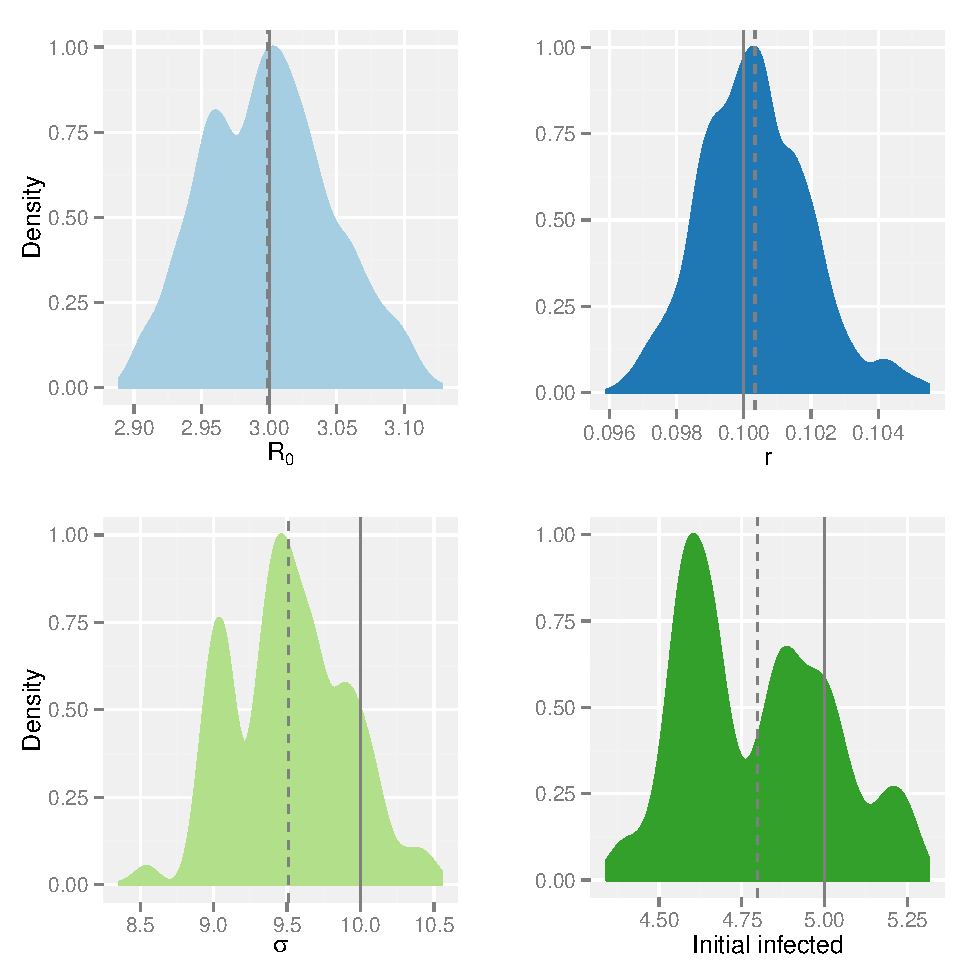
\includegraphics[width=0.8\textwidth]{./images/if2kernels.pdf}
        \caption{Kernel estimates for four essential system parameters. True values are indicated by dashed lines. \label{if2kernelplot}}
    \end{figure}
